\documentclass[12 pt]{article}
\usepackage{graphicx}

\begin{document}

\title{Informe Escrito\\Proyecto: Moogle! }
\author{Amalia Beatriz Valiente Hinojosa\\ C-112.} 
\date{} 
\maketitle

\begin{center}
     Universidad de la Habana: \\ 
     Facultad de Matemática y
Computación.\\ 
\end{center}

\begin{figure}[h] 
    \begin{center} 
        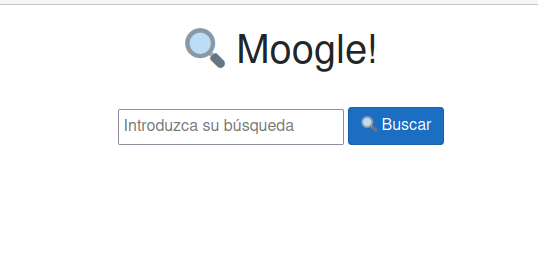
\includegraphics[width = 1 \linewidth]{foto.png} 
    \end{center}
\end{figure}


\newpage

\section{¿Qué es Moogle!?} 
Moogle! es una aplicación cuyo propósito es buscar
inteligentemente y de forma eficiente un texto en un conjunto de documentos.
\\Para su funcionamiento fue emplado el modelo de espacio vectorial, un modelo
algebráico utilizado, entre otras cosas, para el cálculo de relevancia de
información otorgando cierto valor de similitud entre los documentos y la
consulta.

\newpage
\section{Funcionamiento:} 
El modelo de espacio vectorial se divide en una serie
de pasos que permite encontrar los documentos con mayor similitud con la
consulta que se realice.\\El primer paso tenido de cada cuya estructura consiste
en guardar el condocumento en un diccionario es de la siguiente forma:\\

\begin{figure}[h] 
    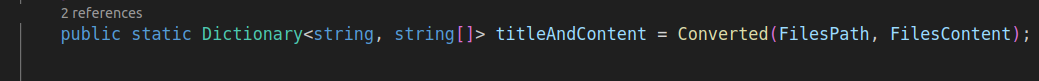
\includegraphics[width = 0.9\linewidth]{titleAndContent.png} 
\end{figure}


\vspace{0.6 cm}

Una vez guardado el contenido de cada documento, se halla la fecuencia de
cada término de cada documento (Term Frequency), que es la primera parte
necesaria para calcular el peso de cada palabra.\\
\\
Para calcular la frecuencia de cada término se emplea la siguiente fórmula:

\begin{equation}
    tf_{t,d} = \frac{freq_{t,d}}{maxf req_d}
\end{equation}

\large Donde:
\begin{itemize}
    \item \small \textbf{tf} (t,d) = la frecuencia del término t en el documento d.
    \item \small \textbf{freq} freq (t,d) = la cantidad de veces que se repite el
    término t n el documento d.
    \item \small \textbf{maxfreq} (d) = el término del documento que más se repite
    en este. 
\end{itemize}

\begin{figure}[h]
	Ahora, los documentos con el tf de cada palabra pasarán a estar
	almacenados en un nuevo diccionario:\\
	\newline
	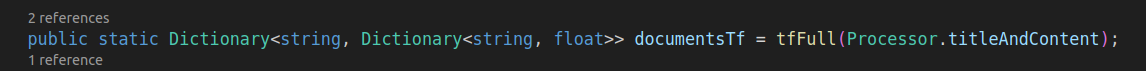
\includegraphics[width =0.9 \linewidth] {TF.png}
\end{figure}

El segundo paso para encontrar el peso de cada palabra es calcular la
frequencia inversa de cada palabra (Inverse Document Frequency) que se halla
mediante la fórmula:

\begin{equation}
    idf_i = \log_{10} (\frac{N}{n_i})
\end{equation}

Donde:
\begin{itemize}
    \item \small \textbf{idf} (i) = frecuencia inversa del término i.
    \item \small \textbf{N} = cantidad de documentos que se encuentran en la
    base de datos.
    \item \small \textbf{n} (i) = cantidad de documentos en los que se
    encuenta el término i.
\end{itemize}

\vspace{0.5 cm}
Esta nueva información se almacena en un tercer diccionario, para posteriormente hallar el peso de cada palabra de los documentos al calcular:

\begin{equation}
    W_{t,d} = tf_{t,d} \times idf_t
\end{equation}

Donde:
\begin{itemize}
    \item \small \textbf{W} (t,d) = peso del término t en el documento d.
\end{itemize}
 \vspace{1 cm}
   Para calcular el peso de las palabras de la query se usa la fórmula: 
 \begin{equation}
    QW_i = (b+(1-b)\cdot \frac{f req_i}{maxf req}) \times idf_i
 \end{equation}

 Donde:
 \begin{itemize}
  \item \small \textbf{QW} (i) = peso del término i de la query. 
 \end{itemize}
 \vspace{0.5 cm}

  Una vez que se obtiene el peso de cada palabra, tanto de los documentos
 como de la query, se procede a evaluar el valor de la similitud entre los
 documentos y la query usando la fórmula de \underline{similitud del coseno}:

 \begin{equation}
    sim(d_j,q) = \frac{\vec{d_j} \cdot \vec{q}}{|\vec{d_j}| \cdot |\vec{q}|}
 \end{equation}

 \begin{center}
    \begin{itemize}
       \item \small el denominador es la multiplicaci\'on de la norma de los vectores documento y query.
    \end{itemize}
 \end{center}

   El peso de cada palabra de los documentos y de cada palabra de la query se almacena en los diccionarios:\
   \newline
\begin{figure}[h]
    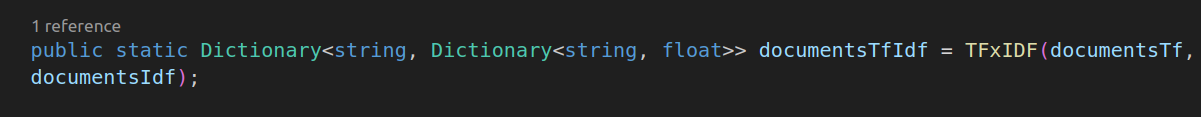
\includegraphics[width=1 \linewidth]{tfIdf.png}
\end{figure}


 \begin{figure}[h]
    y:
  \newline
  \newline
    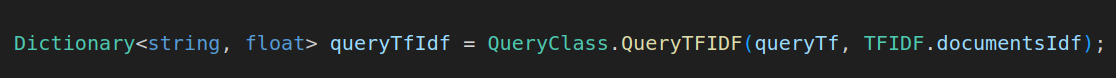
\includegraphics[width = 1 \linewidth]{queryTFIDF.png}
 \end{figure}

 Una vez se obtiene la simlitud del coseno, cada documento es almacenado
 en un diccionario ordenado de menor a mayor valor, y, como resultado de la
 búsqueda, se develven los tres últimos documentos, que son los que tienen mayor
 similitud con la query.
 \newline
 \newline
 Además de los documentos, también se devuelve un
 fragmento del documento en donde aparece al menos una palabra de la query, a
 este fragmento se le denomina \textbf{Snippet}.

\newpage
 \section{Estructura} Este proceso fue llevado a cabo en 4 clases:
 \begin{itemize} \item \textbf{Processor:} En esta clase se normalizan los
 documentos y se separan y almacenan en diccionarios. \item \textbf{Query:}En
 esta clase se normaliza el contenido de la query y se calcula el peso de las
 palabras contenidas en ella. \item \textbf{TF-IDF:} En esta clase se halla el
 peso de las palabras de los documtos, la similitud entre los documentos y la
 query y el snippet. \item \textbf{Moogle:} En esta se encuentra el método
 principal que devuelve el resultado de la búsqueda. \end{itemize}






 \newpage
 \section{Manual}
    Para efectuar una consulta en Moogle! basta con escribir
    fragmentos o el nombre del documento que se quiere encontrar y dar click en
    el botón azul que se encuentra a la derecha de la barra de consulta.\\
\begin{figure}[h]
    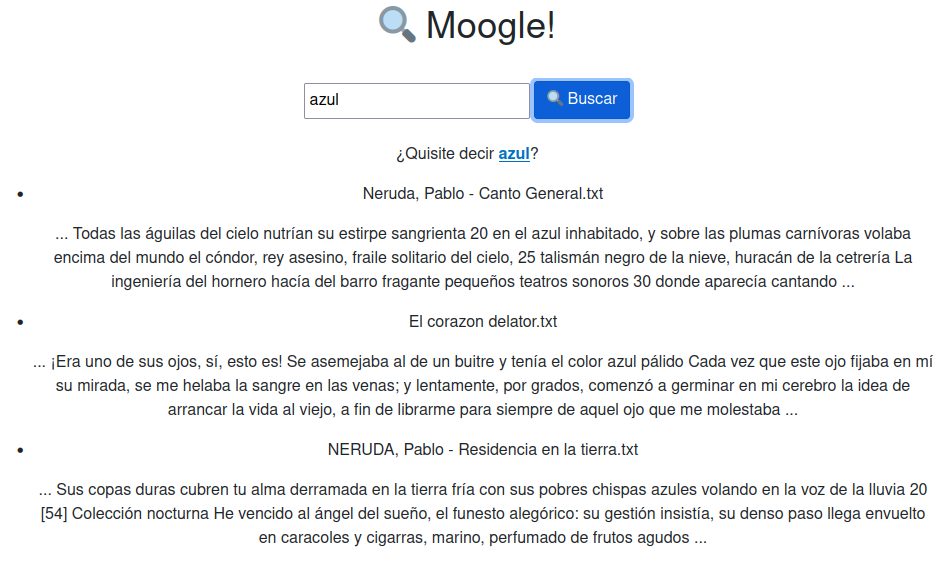
\includegraphics[width = 1.2 \linewidth]{ejemplo.png}
\end{figure}
\end{document}